\documentclass{beamer}

% \usepackage{beamerthemesplit} // Activate for custom appearance

\title{Principal Component Analysis}
\author{Frank Wood}
\date{\today}

\newcommand{\comment}[1]{}
\newcommand{\ponedec}{\mathcal{P}^\downarrow_1}
\newcommand{\pone}{\mathcal{P}_1}
\newcommand{\rank}[1]{\mathrm{RANK}\left[#1\right]}
\newcommand{\E}[1]{\mathrm{E}\left[#1\right]}
\newcommand{\py}{\mathcal{PY}}
\newcommand{\iid}{iid.}
\newcommand{\drawiid}{\stackrel{\text{iid}}{\sim}}
\newcommand{\vect}[1]{\mathbf{#1}}
\newcommand{\indicator}[1]{\text{I}\left[ #1 \right]}
\newcommand{\pdcoag}{PD(d_1,0)-\text{COAG}}
\newcommand{\todo}{\textbf{*TODO*}}
\newcommand{\igram}{\text{$\infty$-gram}}
\newcommand{\Prob}{\text{P}}

\def\mm{sequence memoizer }
\def\MM{SM }

\def\pibf{{\boldsymbol{\pi}}}
\def\kapbf{\boldsymbol{\kappa}}
\def\taubf{\boldsymbol{\tau}}
\def\alphabf{\boldsymbol{\alpha}}
\def\thebf{\boldsymbol{\theta}}
\def\Sigmabf{\boldsymbol{\Sigma}}
\def\Lambdabf{\boldsymbol{\Lambda}}

\def\epsilonbf{\boldsymbol{\epsilon}}
\def\betabf{\boldsymbol{\beta}}
\def\phibf{\boldsymbol{\phi}}
\def\gammabf{\boldsymbol{\gamma}}

\def\pbf{\mathbf{p}}
\def\qbf{\mathbf{q}}
\def\sbf{\mathbf{s}}
\def\tbf{\mathbf{t}}
\def\ybf{\mathbf{y}}
\def\wbf{\mathbf{w}}
\def\xbf{\mathbf{x}}
\def\rbf{\mathbf{r}}
\def\tbf{\mathbf{t}}
\def\abf{\mathbf{a}}
\def\kbf{\mathbf{k}}
\def\Zbf{\mathbf{Z}}
\def\Xbf{\mathbf{X}}
\def\Sbf{\mathbf{S}}
\def\Bbf{\mathbf{B}}
\def\Abf{\mathbf{A}}

\def\0bf{\mathbf{0}}
\def\Ibf{\mathbf{I}}
\def\phibf{\mathbf{\phi}}
\def\Phibf{\mathbf{\Phi}}
\def\disteq{{\stackrel{D}{=}}}
\def\EE{{\mathbb{E}}}

\def\phiv{\varphi}
\def\phivbf{\boldsymbol{\varphi}}

\def\Ocal{\mathcal{O}}

\DeclareMathOperator*{\Bet}{Beta}
\DeclareMathOperator{\coag}{COAG}
\DeclareMathOperator{\frag}{FRAG}
\DeclareMathOperator*{\rnk}{RANK}
\DeclareMathOperator*{\gem}{GEM}
\DeclareMathOperator*{\pd}{PD}
\DeclareMathOperator*{\gd}{GDir}
\DeclareMathOperator*{\Dir}{Dir}
\DeclareMathOperator*{\N}{N}
\DeclareMathOperator*{\Ave}{\mathbb{E}}
\DeclareMathOperator*{\Var}{Var}
\DeclareMathOperator*{\cov}{cov}
\DeclareMathOperator*{\tr}{tr}

\begin{document}

\frame{\titlepage {\tiny This lecture borrows and {\em quotes} from Joliffe's Principle Component Analysis book.  Go buy it!}}

%\section[Outline]{}
%\frame{\tableofcontents}

%\section{Bayesian Analysis}
%\subsection{Single Parameter Model}
\frame[t] {% slide 1
 \frametitle{Principal Component Analysis}
\begin{quote}
The central idea of principal component analysis (PCA) is to reduce the dimensionality of a data set consisting of a large number of interrelated variables, while retaining as much as possible of the variation present in the data set.  This is achieved by transforming to a new set of variables, the principal components (PCs), which are uncorrelated, and which are ordered so that the first {\em few} retain most of the variation present in {\em all} of the original variables. [Jolliffe, Pricipal Component Analysis, $2^{nd}$ edition]
\end{quote}
}
\section{Principal Component Analysis in Pictures}

\frame[t] {% slide 1
 \frametitle{{\em Data} distribution (inputs in regression analysis)}
\begin{figure}[htbp]
\begin{center}
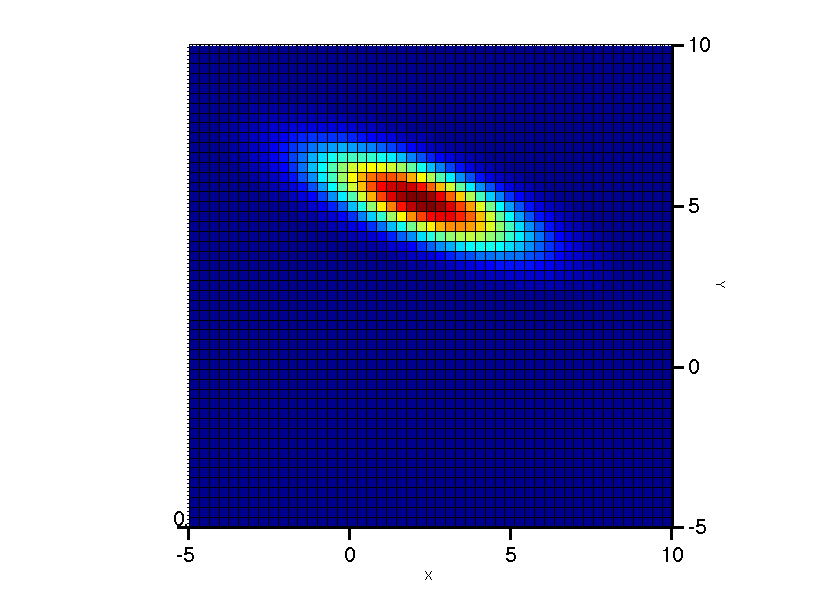
\includegraphics[width=.9\linewidth]{matlab/gaussian_pdf.png}
\caption{Gaussian PDF}
\label{gaussian_pdf.png}
\end{center}
\end{figure}
}

\frame[t] {% slide 1
 \frametitle{Uncorrelated projections of principal variation}
\begin{figure}[htbp]
\begin{center}
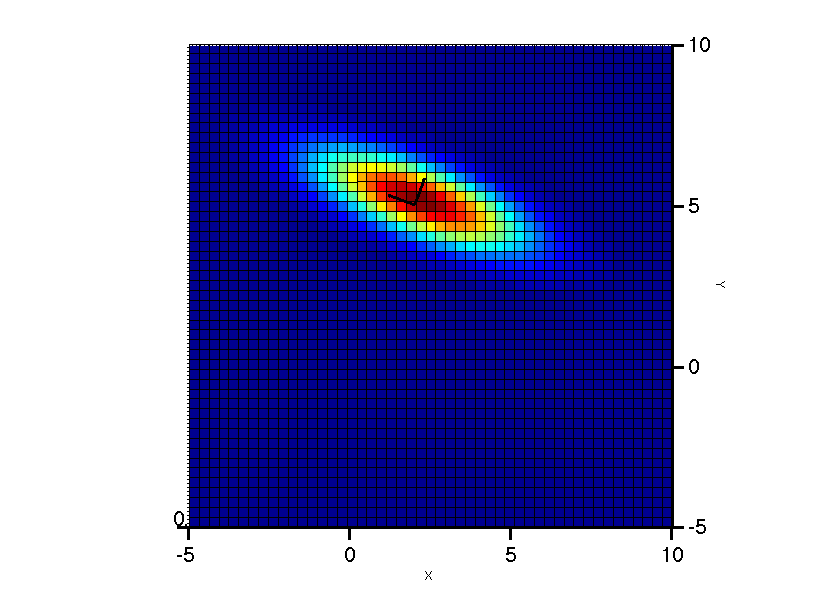
\includegraphics[width=.9\linewidth]{matlab/gaussian_pdf_pca_axis.png}
\caption{Gaussian PDF with PC eigenvectors}
\label{gaussian_pdf_pca_axis.png}
\end{center}
\end{figure}
}


\frame[t] {% slide 1
 \frametitle{PCA rotation}
\begin{figure}[htbp]
\begin{center}
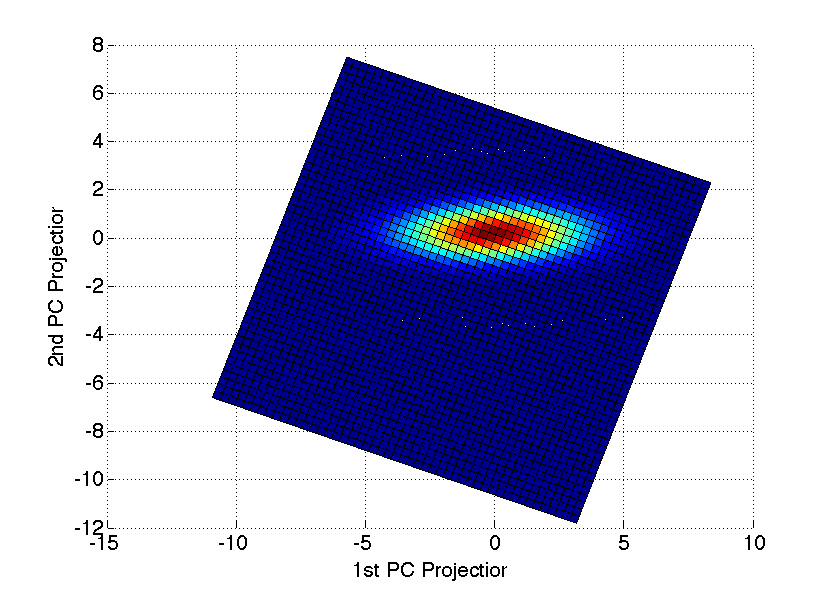
\includegraphics[width=.9\linewidth]{matlab/gaussian_pdf_rotated.png}
\caption{PCA Projected Gaussian PDF}
\label{gaussian_pdf_rotated.png}
\end{center}
\end{figure}
}


\frame[t] {% slide 1
 \frametitle{PCA in a nutshell}
\begin{block}{Notation}
\begin{itemize}
\item $\xbf$ is a vector of $p$ random variables
\item $\alphabf_k$ is a vector of $p$ constants
\item $\alphabf_k'\xbf = \sum_{j=1}^p \alpha_{kj}x_j$
\end{itemize}
\end{block}

\begin{block}{Procedural description}
\begin{itemize}
\item Find linear function of $\xbf$, $\alphabf_1'\xbf$ with maximum variance.
\item Next find another linear function of $\xbf$, $\alphabf_2'\xbf$, uncorrelated with $\alphabf_1'\xbf$ maximum variance.
\item Iterate.
\end{itemize}
\end{block}

\begin{block}{Goal}
It is hoped, in general, that most of the variation in $\xbf$ will be accounted for by $m$ PC's where $m<<p$.
\end{block}

}


\frame[t] {% slide 1
 \frametitle{Derivation of PCA}
\begin{block}{Assumption and More Notation}
\begin{itemize}
\item $\Sigmabf$ is the {\em known} covariance matrix for the random variable $\xbf$
\item Foreshadowing : $\Sigmabf$ will be replaced with $\Sbf$, the sample covariance matrix, when $\Sigmabf$ is unknown.
\end{itemize}
\end{block}

\begin{block}{Shortcut to solution}
\begin{itemize}
\item For $k=1,2,\ldots,p$ the $k^{th}$ PC is given by $z_k = \alphabf_k'\xbf$ where $\alphabf_k$ is an eigenvector of $\Sigmabf$ corresponding to its $k^{th}$ largest eigenvalue $\lambda_k$.
\item If $\alphabf_k$ is chosen to have unit length (i.e.~$\alphabf_k'\alphabf_k=1$) then $\Var(z_k) = \lambda_k$
\end{itemize}
\end{block}


}

\frame[t] {% slide 1
 \frametitle{Derivation of PCA}
\begin{block}{First Step}
\begin{itemize}
\item Find $\alphabf_k'\xbf$ that maximizes $\Var(\alphabf_k'\xbf) = \alphabf_k'\Sigmabf\alphabf_k$
\item Without constraint we could pick a very big $\alphabf_k$.
\item Choose normalization constraint, namely $\alphabf_k'\alphabf_k = 1$ (unit length vector).
\end{itemize}
\end{block}

\begin{block}{Constrained maximization - method of Lagrange multipliers}
\begin{itemize}
\item To maximize $\alphabf_k'\Sigmabf\alphabf_k$ subject to $\alphabf_k'\alphabf_k = 1$ we use the technique of Lagrange multipliers.  We maximize the function 
\begin{equation*}
\alphabf_k'\Sigmabf\alphabf_k - \lambda(\alphabf_k'\alphabf_k -1)
\end{equation*}
w.r.t. to $\alphabf_k$ by differentiating w.r.t. to $\alphabf_k$. 
\end{itemize}
\end{block}

}

\frame[t] {% slide 1
 \frametitle{Derivation of PCA}

\begin{block}{Constrained maximization - method of Lagrange multipliers}
\begin{itemize}
\item This results in 
\begin{eqnarray*}
\frac{d}{d\alphabf_k}\left(\alphabf_k'\Sigmabf\alphabf_k - \lambda_k(\alphabf_k'\alphabf_k -1)\right) &=& 0 \\
\Sigmabf\alphabf_k - \lambda_k\alphabf_k &=& 0 \\
\Sigmabf\alphabf_k &=&  \lambda_k\alphabf_k
\end{eqnarray*}
\item This should be recognizable as an eigenvector equation where $\alphabf_k$ is an eigenvector of $\Sigma_bf$ and $\lambda_k$ is the associated eigenvalue.
\item Which eigenvector should we choose?
\end{itemize}
\end{block}
}


\frame[t] {% slide 1
 \frametitle{Derivation of PCA}

\begin{block}{Constrained maximization - method of Lagrange multipliers}
\begin{itemize}
\item If we recognize that the quantity to be maximized 
 \begin{eqnarray*}
\alphabf_k'\Sigmabf\alphabf_k = \alphabf_k'\lambda_k\alphabf_k = \lambda_k\alphabf_k'\alphabf_k = \lambda_k
\end{eqnarray*}
then we should choose $\lambda_k$ to be as big as possible.  So, calling $\lambda_1$ the largest eigenvector of $\Sigma$ and $\alphabf_1$ the corresponding eigenvector then the solution to 
\begin{eqnarray*}
\Sigmabf\alphabf_1 &=&  \lambda_1\alphabf_1
\end{eqnarray*}
is the $1^{st}$ principal component of $\xbf$.
\item In general $\alphabf_k$ will be the $k^{th}$ PC of $\xbf$ and $\Var(\alphabf'\xbf) = \lambda_k$
\item We will demonstrate this for $k=2$, $k>2$ is more involved but similar.
\end{itemize}
\end{block}
}

\frame[t] {% slide 1
 \frametitle{Derivation of PCA}

\begin{block}{Constrained maximization - more constraints}
\begin{itemize}
\item The second PC, $\alphabf_2\xbf$ maximizes $\alphabf_2\Sigma\alphabf_2$ subject to being uncorrelated with $\alphabf_1\xbf$.
\item The uncorrelation constraint can be expressed using any of these equations

\begin{eqnarray*}\cov(\alphabf_1'\xbf, \alphabf_2'\xbf) &=& \alphabf_1'\Sigmabf \alphabf_2 = \alphabf_2'\Sigmabf \alphabf_1 = \alphabf_2'\lambda_1\alphabf_1' \\&=& \lambda_1\alphabf'_2\alphabf = \lambda_1 \alphabf_1'\alphabf_2 = 0\end{eqnarray*}
\item Of these, if we choose the last we can write an Langrangian to maximize $\alphabf_2$
\begin{eqnarray*}
\alphabf_2'\Sigmabf \alphabf_2 - \lambda_2(\alphabf_2'\alphabf_2-1)-\phi\alphabf_2' \alphabf_1
\end{eqnarray*}

\end{itemize}
\end{block}
}

\frame[t] {% slide 1
 \frametitle{Derivation of PCA}

\begin{block}{Constrained maximization - more constraints}
\begin{itemize}
\item Differentiation of this quantity  w.r.t.~$\alphabf_2$ (and setting the result equal to zero) yields
\begin{eqnarray*}
\frac{d}{d\alphabf_2}\left(\alphabf_2'\Sigmabf \alphabf_2 - \lambda_2(\alphabf_2'\alphabf_2-1)-\phi\alphabf_2' \alphabf_1\right) = 0 \\
\Sigmabf \alphabf_2 - \lambda_2\alphabf_2-\phi\alphabf_1 = 0
\end{eqnarray*}
\item If we left multiply $\alphabf_1$ into this expression
\begin{eqnarray*}
\alphabf_1'\Sigmabf \alphabf_2 - \lambda_2\alphabf_1'\alphabf_2-\phi\alphabf_1'\alphabf_1 = 0 \\
0 - 0 -\phi 1 = 0
\end{eqnarray*}
then we can see that $\phi$ must be zero and that when this is true that we are left with 
\[\Sigmabf \alphabf_2 - \lambda_2\alphabf_2 = 0\]
\end{itemize}
\end{block}
}

\frame[t] {% slide 1
 \frametitle{Derivation of PCA}
Clearly 
\[\Sigmabf \alphabf_2 - \lambda_2\alphabf_2 = 0\]
 is another eigenvalue equation and the same strategy of choosing $\alpha_2$ to be the  eigenvector associated with the second largest eigenvalue yields the second PC of $\xbf$, namely $\alphabf_2'\xbf$.
\bigskip

This process can be repeated for $k=1\ldots p$ yielding up to $p$ different eigenvectors of $\Sigmabf$ along with the corresponding eigenvalues $\lambda_1, \ldots \lambda_p$.
\bigskip

Furthermore, the variance of each of the PC's are given by
\[\Var[\alphabf_k'\xbf] = \lambda_k, \qquad k = 1,2,\ldots,p\]

}


\frame[t] {% slide 1
 \frametitle{Properties of PCA}
For any integer $q, 1 \leq q \leq p,$ consider the orthonormal linear transformation 
\[ \ybf = \Bbf'\xbf\] 
where $\ybf$ is a $q$-element vector and $\Bbf'$ is a $q\times p$ matrix, and let $\Sigmabf_y = \Bbf'\Sigmabf\Bbf$ be the variance-covariance matrix for $\ybf$.  Then the trace of $\Sigmabf_y$, denoted $\tr(\Sigmabf_y)$, is maximized by taking $\Bbf = \Abf_q,$ where $\Abf_q$ consists of the first $q$ columns of $\Abf$. 
\bigskip

What this means is that if you want to choose a lower dimensional projection of $\xbf$, the choice of $\Bbf$ described here is probably a good one.  It maximizes the (retained) variance of the resulting variables.
\bigskip

In fact, since the projections are uncorrelated, the percentage of variance accounted for by retaining the first $q$ PC's is given by
\[ \frac{\sum_{k=1}^{q} \lambda_k}{\sum_{k=1}^{p} \lambda_k} \times 100\]
}

\frame[t] {% slide 1
 \frametitle{PCA using the sample covariance matrix}
If we recall that the sample covariance matrix (an unbiased estimator for the covariance matrix of $\xbf$) is given by 
\[\Sbf = \frac{1}{n-1} \Xbf'\Xbf\]
where $\Xbf$ is a $(n\times p)$ matrix with $(i,j)th$ element $(x_{ij} - \bar x_j)$ (in other words, $\Xbf$ is a zero mean design matrix).
\bigskip

We construct the matrix $\Abf$ by combining the $p$ eigenvectors of $\Sbf$ (or eigenvectors of $\Xbf'\Xbf$ -- they're the same) then we can define a matrix of PC scores
\[\Zbf = \Xbf\Abf\]
Of course, if we instead form $\Zbf$ by selecting the $q$ eigenvectors corresponding to the $q$ largest eigenvalues of $\Sbf$ when forming $\Abf$ then we can achieve an ``optimal'' (in some senses) $q$-dimensional projection of $\xbf$.
}

\frame[t] {% slide 1
 \frametitle{Computing the PCA loading matrix}
Given the sample covariance matrix
\[\Sbf = \frac{1}{n-1} \Xbf'\Xbf\]
the most straightforward way of computing the PCA loading matrix is to utilize the singular value decomposition of $\Sbf = \Abf'\Lambdabf\Abf$ where $\Abf$ is a matrix consisting of the eigenvectors of $\Sbf$ and $\Lambdabf$ is a diagonal matrix whose diagonal elements are the eigenvalues corresponding to each eigenvector.
\bigskip

Creating a reduced dimensionality projection of $\Xbf$ is accomplished by selecting the $q$ largest eigenvalues in $\Lambdabf$ and retaining the $q$ corresponding eigenvectors from $\Abf$
}



\section{Sample Covariance Matrix PCA}


\frame[t] {% slide 1
 \frametitle{Sample Covariance Matrix PCA}
\begin{figure}[htbp]
\begin{center}
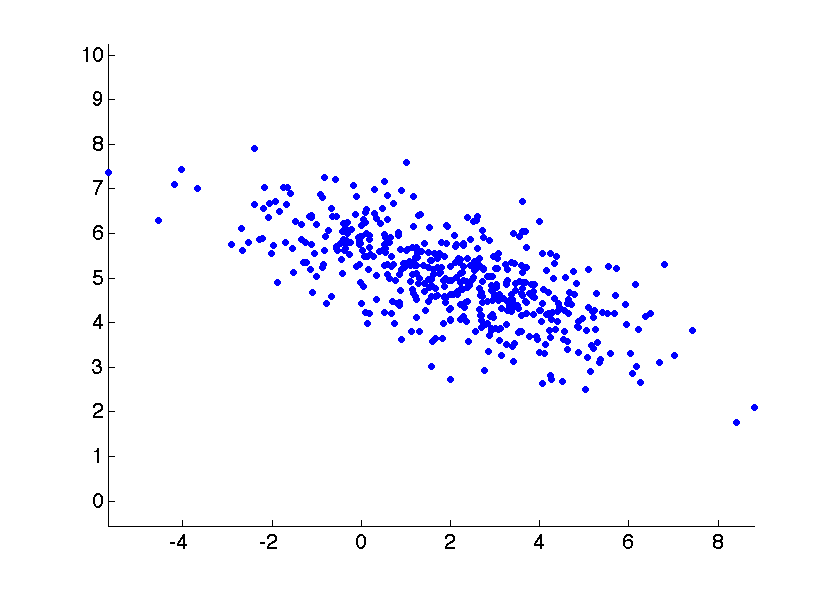
\includegraphics[width=.9\linewidth]{matlab/2d_samples.png}
\caption{Gaussian Samples}
\label{2d_samples.png}
\end{center}
\end{figure}
}

\frame[t] {% slide 1
 \frametitle{Sample Covariance Matrix PCA}
\begin{figure}[htbp]
\begin{center}
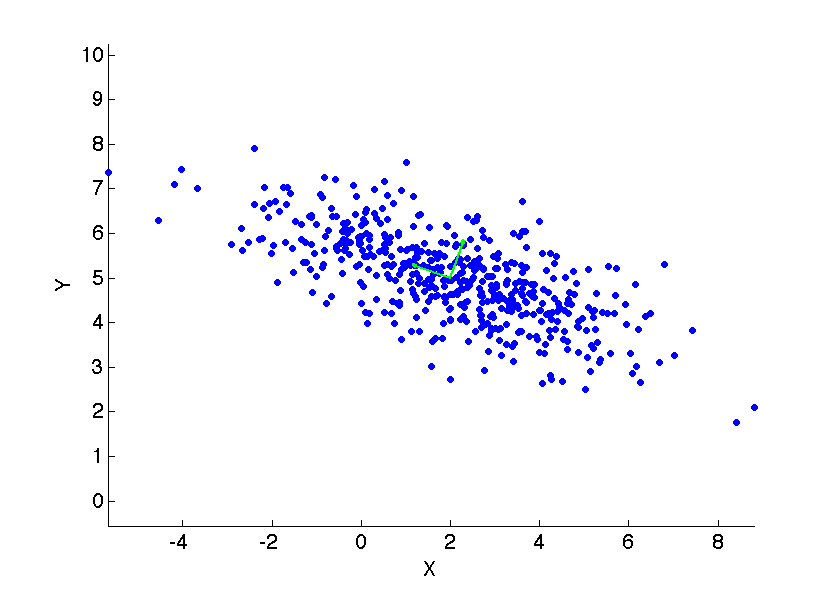
\includegraphics[width=.9\linewidth]{matlab/2d_samples_pca_axis.png}
\caption{Gaussian Samples with eigenvectors of sample covariance matrix}
\label{2d_samples_pca_axis.png}
\end{center}
\end{figure}
}


\frame[t] {% slide 1
 \frametitle{Sample Covariance Matrix PCA}
\begin{figure}[htbp]
\begin{center}
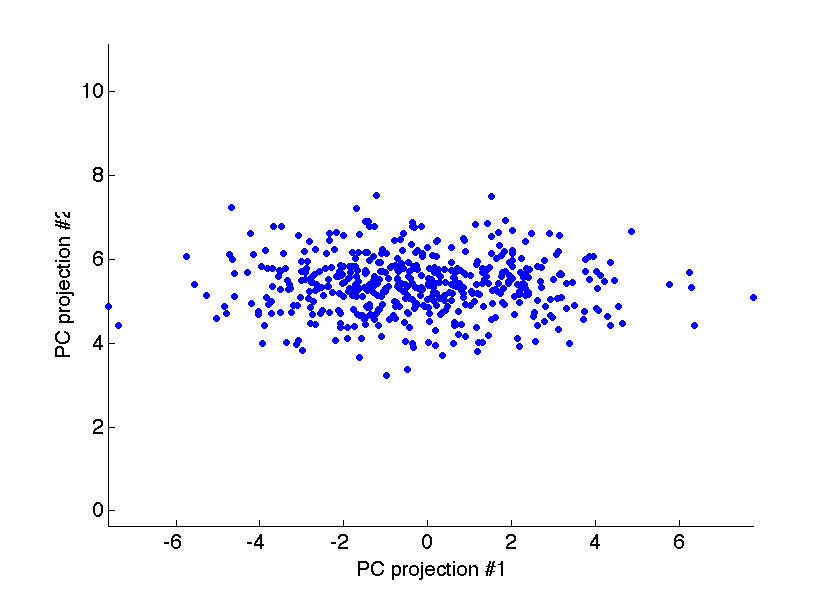
\includegraphics[width=.9\linewidth]{matlab/2d_samples_rotated.png}
\caption{PC projected samples}
\label{2d_samples_rotated.png}
\end{center}
\end{figure}
}

\frame[t] {% slide 1
 \frametitle{Sample Covariance Matrix PCA}
\begin{figure}[htbp]
\begin{center}
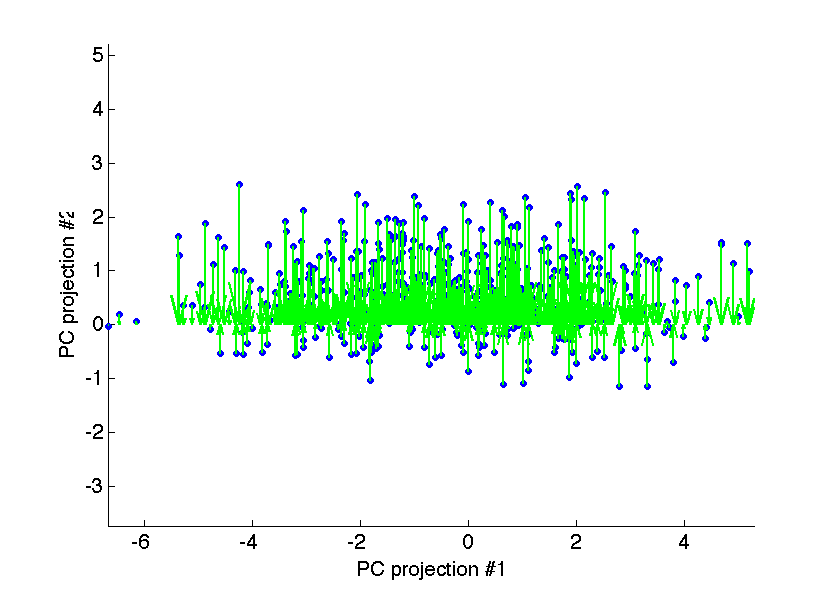
\includegraphics[width=.9\linewidth]{matlab/pc_projection.png}
\caption{PC dimensionality reduction step}
\label{pc_projection.png}
\end{center}
\end{figure}
}

\frame[t] {% slide 1
 \frametitle{Sample Covariance Matrix PCA}
\begin{figure}[htbp]
\begin{center}
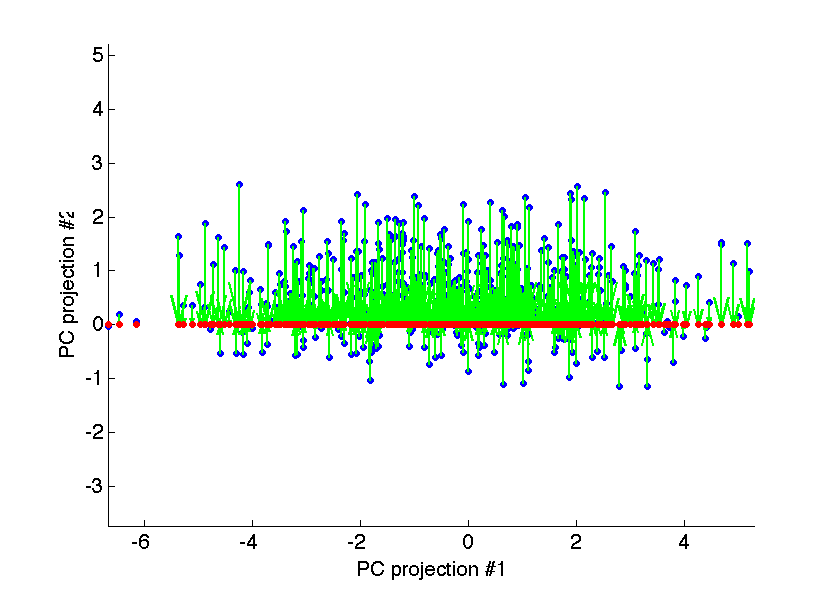
\includegraphics[width=.9\linewidth]{matlab/pc_projected.png}
\caption{PC dimensionality reduction step}
\label{pc_projected.png}
\end{center}
\end{figure}
}

\section{PCA Linear Regression}

\frame[t] {% slide 1
 \frametitle{PCA in linear regression}
 PCA is useful in linear regression in several ways
\begin{itemize}
\item  Identification and elimination of multicolinearities in the data.
\item Reduction in the dimension of the input space leading to fewer parameters and ``easier'' regression.
\item Related to the last point, the variance of the regression coefficient estimator is minimized by the PCA choice of basis.
\end{itemize}
We will consider the following example.
\begin{itemize}
\item $\xbf \sim \N\left([2 \; 5],\left[ 
\begin{array}{cc}
4.5  & -1.5    \\
 -1.5 & 1.0    
\end{array}
\right]\right)$
\item $\ybf = \Xbf[-1 \; 2] '$ when no colinearities are present (no noise)
\item $x_{i3} =  .8x_{i1} + .5x_{i2}$ {\em imposed} colinearity
\end{itemize}
}

\frame[t] {% slide 1
 \frametitle{Noiseless Linear Relationship with No Colinearity}
\begin{figure}[htbp]
\begin{center}
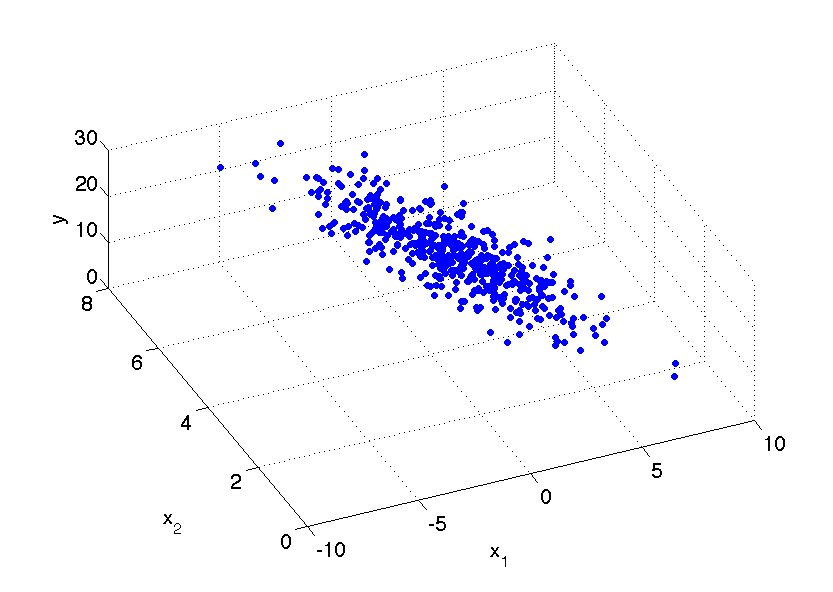
\includegraphics[width=.9\linewidth]{matlab/2d_regression.png}
\caption{$\ybf = \xbf[-1 \; 2] '+ 5, \xbf \sim \N([2 \; 5],\left[ 
\begin{array}{cc}
4.5  & -1.5    \\
 -1.5 & 1.0    
\end{array}
\right])$}
\label{fig:2d_regression}
\end{center}
\end{figure}
}


\frame[t] {% slide 1
 \frametitle{Noiseless Planar Relationship}
\begin{figure}[htbp]
\begin{center}
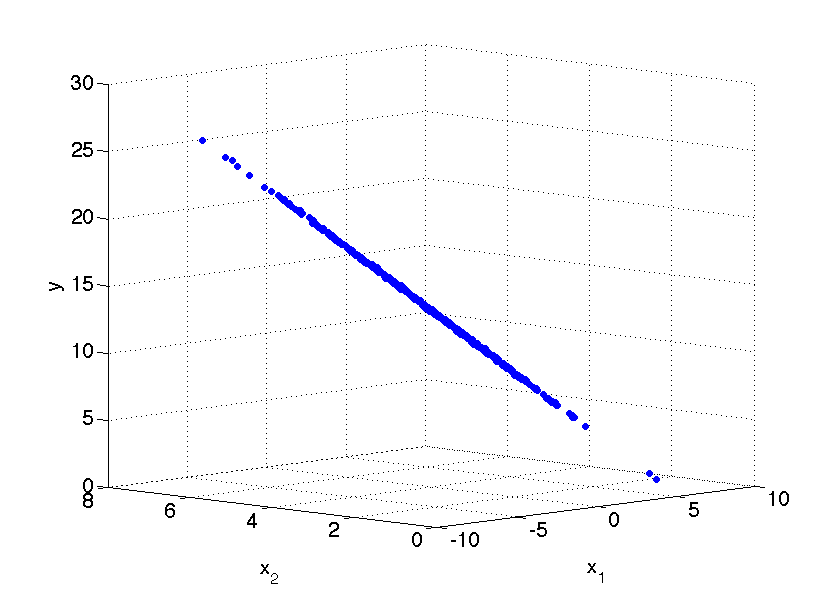
\includegraphics[width=.9\linewidth]{matlab/2d_regression_flat.png}
\caption{$\ybf = \xbf[-1 \; 2] '+ 5, \xbf \sim \N([2 \; 5],\left[ 
\begin{array}{cc}
4.5  & -1.5    \\
 -1.5 & 1.0    
\end{array}
\right])$}
\label{2d_regression_flat.png}
\end{center}
\end{figure}
}

\subsection{Multicolinearity}

\frame[t] {% slide 1
 \frametitle{Projection of colinear data}
The figures before showed the data without the third colinear design matrix column.  Plotting such data is not possible, but it's colinearity is obvious by design.
\bigskip

When PCA is applied to the design matrix of rank $q$ less than $p$ the number of positive eigenvalues discovered is equal to $q$ the true rank of the design matrix.   
\bigskip

If the number of PC's retained is larger than $q$ (and the data is perfectly colinear, etc.) {\em all} of the variance of the data is retained in the low dimensional projection.
\bigskip

In this example, when PCA is run on the design matrix of rank 2, the resulting projection back into two dimensions has exactly the same distribution as before.
}

\frame[t] {% slide 1
 \frametitle{Projection of colinear data}
\begin{figure}[htbp]
\begin{center}
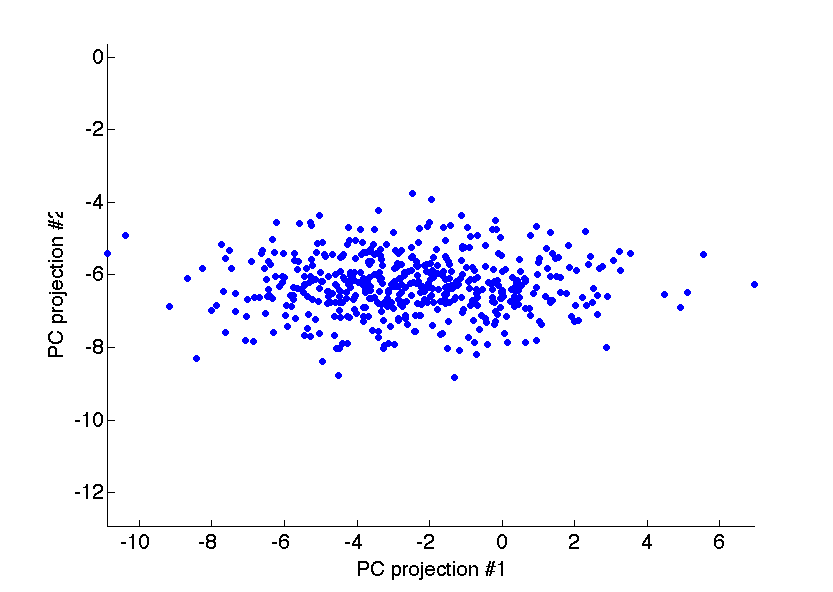
\includegraphics[width=.9\linewidth]{matlab/pca_conlinearity_removal.png}
\caption{Projection of multi-colinear data onto first two PC's}
\label{pca_conlinearity_removal.png}
\end{center}
\end{figure}
}

\frame[t] {% slide 1
 \frametitle{Reduction in regression coefficient estimator variance}
If we take the standard regression model
\[ \ybf = \Xbf\betabf + \epsilonbf\]
And consider instead the PCA rotation of $\Xbf$ given by 
\[\Zbf = \Zbf\Abf\]
then we can rewrite the regression model in terms of the PC's
\[\ybf = \Zbf\gammabf + \epsilonbf.\]
We can also consider the reduced model
\[\ybf = \Zbf_q\gammabf_q + \epsilonbf_q\]
where only the first $q$ PC's are retained.
}

\frame[t] {% slide 1
 \frametitle{Reduction in regression coefficient estimator variance}
If we rewrite the regression relation as
\[\ybf = \Zbf\gammabf + \epsilonbf.\]
Then we can, because $\Abf$ is orthogonal, rewrite
\[\Xbf\betabf = \Xbf\Abf\Abf'\betabf = \Zbf\gammabf\]
where $\gammabf = \Abf'\beta$.
\bigskip

Clearly using least squares (or ML) to learn $\hat \betabf = \Abf \hat \gammabf$ is equivalent to learning $\hat \betabf$ directly.  
\bigskip

And, like usual, 
\[\hat \gammabf = (\Zbf'\Zbf)^{-1}\Zbf'\ybf\]
so $\hat \betabf = \Abf (\Zbf'\Zbf)^{-1}\Zbf'\ybf$
}

\frame[t] {% slide 1
 \frametitle{Reduction in regression coefficient estimator variance}
 Without derivation we note that the variance-covariance matrix of $\hat \betabf$ is given by
 \[ \Var(\hat \betabf) = \sigma^2\sum_{k=1}^p l_k^{-1}\abf_k\abf_k'\]
 where $l_k$ is the $k^{th}$ largest eigenvalue of $\Xbf'\Xbf$, $\abf_k$ is the $k^{th}$ column of $\Abf$, and $\sigma^2$ is the observation noise variance, i.e.~$\epsilonbf \sim \N(\0bf,\sigma^2\Ibf)$
 \bigskip
 
 This sheds light on how multicolinearities produce large variances for the elements of $\hat \betabf$.  If an eigenvector $l_k$ is small then the resulting variance of the estimator will be large.
 \bigskip
 

}

\frame[t] {% slide 1
 \frametitle{Reduction in regression coefficient estimator variance}

 
 One way to avoid this is to ignore those PC's that are associated with small eigenvalues, namely, use  biased estimator
 \[\tilde \betabf =\sum_{k=1}^m l_k^{-1}\abf_k\abf_k'\Xbf'\ybf\]

where $l_{1:m}$ are the large eigenvalues of $\Xbf'\Xbf$ and $l_{m+1:p}$ are the small.
 
 
  \[ \Var(\tilde \betabf ) = \sigma^2\sum_{k=1}^m l_k^{-1}\abf_k\abf_k'\]

This is a biased estimator, but, since the variance of this estimator is smaller it is possible that this could be an advantage.
\bigskip

Homework: find the bias of this estimator.  Hint: use the spectral decomposition of $\Xbf'\Xbf$.

}

\section{PCA Limitations}

\frame[t] {% slide 1
 \frametitle{Problems with PCA}
PCA is not without its problems and limitations
\begin{itemize}
\item PCA assumes approximate normality of the input space distribution
\begin{itemize}
\item PCA may still be able to produce a ``good'' low dimensional projection of the data even if the data isn't normally distributed
\end{itemize}
\item PCA may ``fail'' if the data lies on a ``complicated'' manifold
\item PCA assumes that the input data is real and continuous.
\item Extensions to consider
\begin{itemize}
\item Collins et al, A generalization of principal components analysis to the exponential family.
\item Hyv{\\"a}rinen, A. and Oja, E., Independent component analysis: algorithms and applications
\item ISOMAP, LLE, Maximum variance unfolding, etc.
\end{itemize}
\end{itemize}


}



\frame[t] {% slide 1
 \frametitle{Non-normal data}
\begin{figure}[htbp]
\begin{center}
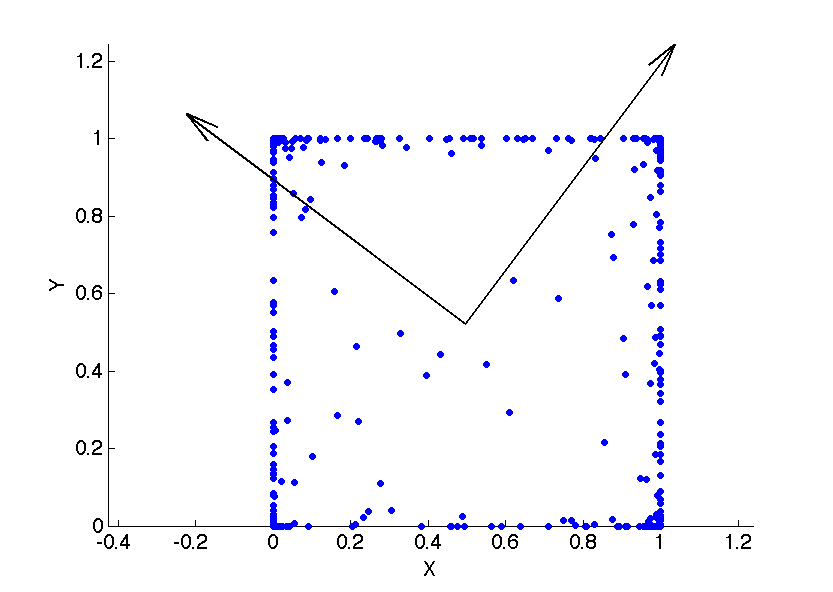
\includegraphics[width=.9\linewidth]{matlab/beta_samples_pca_axis.png}
\caption{2d $\Bet(.1,.1)$ Samples with PC's}
\label{beta_samples_pca_axis.png}
\end{center}
\end{figure}
}


\frame[t] {% slide 1
 \frametitle{Non-normal data}
\begin{figure}[htbp]
\begin{center}
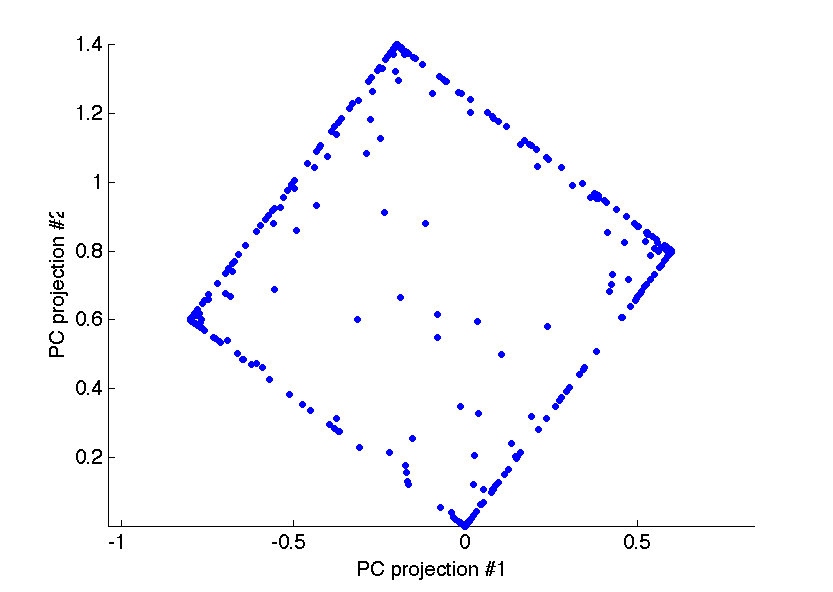
\includegraphics[width=.9\linewidth]{matlab/beta_samples_rotated.png}
\caption{PCA Projected}
\label{beta_samples_rotated.png}
\end{center}
\end{figure}
}






\end{document}
